\chapter{Connecting to BLE device}
\label{ch:connecting_to_ble}

\begin{figure}[htb]
    \centering
	  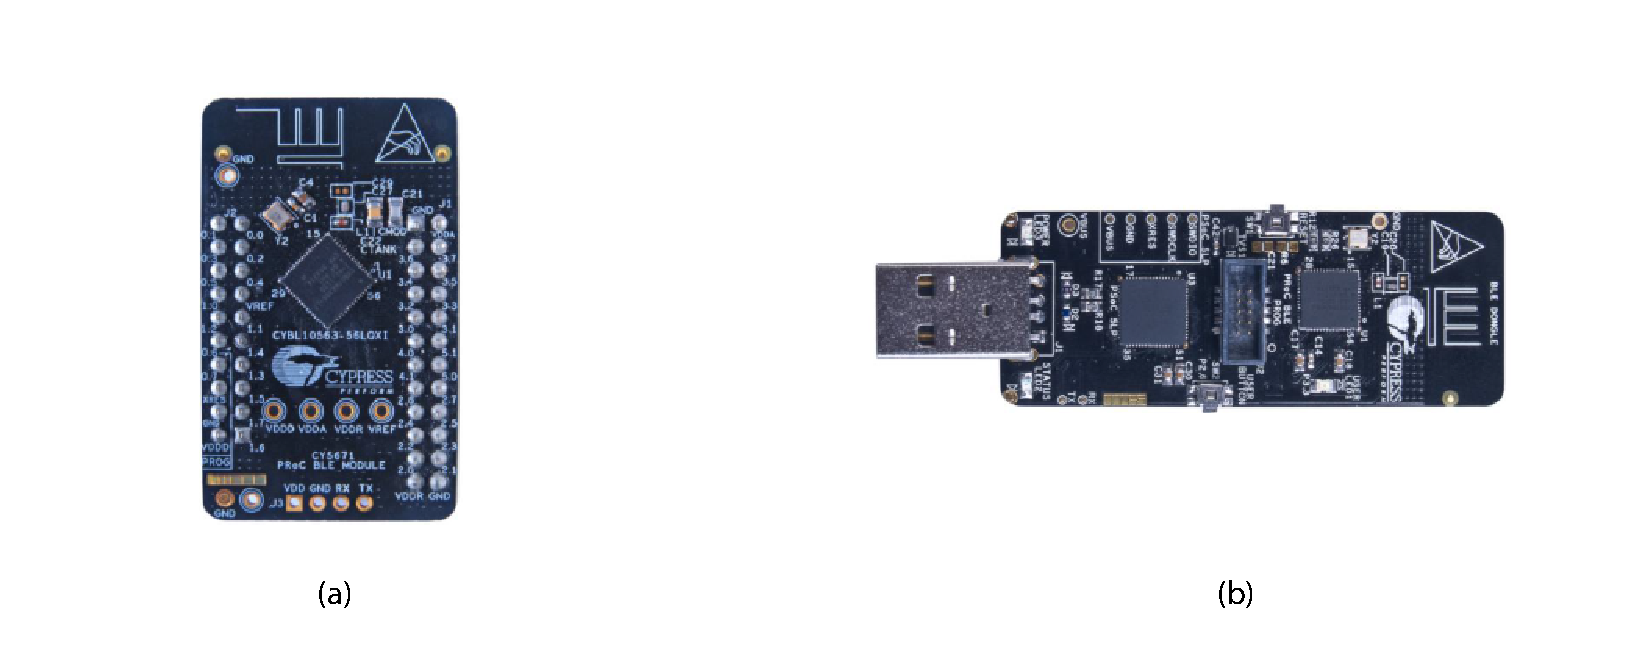
\includegraphics[width=0.8\linewidth]{figures/BLE_module_Dongle.pdf}
	\caption{Hardware needed to establish BLE bridge: (a) BLE module on MU (CY5671), (b) BLE USB dongle (CY5670)}
	\label{fig:ble_hardware}
\end{figure}

Hardware components:
\begin{itemize}
	\item BLE module on MU -- \url{http://www.cypress.com/documentation/development-kitsboards/cy5671-proc-ble-module} 
	\item BLE dongle -- \url{http://www.cypress.com/documentation/development-kitsboards/cy5670-cysmart-usb-dongle} \\
	The purpose of BLE dongle is to provide UART bridge between MU and PC. It can be used for programming MU via BLE Bootloader or for basic serial communication.
\end{itemize}

In order to connect to BLE device on aMussel, the following prerequisites have to be met:
\begin{enumerate}
	\item You need to have BLE dongle configured.
	\item BLE board on MU has to be programmed.
\end{enumerate}

\section{Configuring BLE dongle}

BLE dongle needs to be programmed using MiniProg. The code is provided in \texttt{BLE\_DONGLE} project of PSoC creator \texttt{MU31S-000} workspace.

\begin{figure}[htb]
    \centering
	  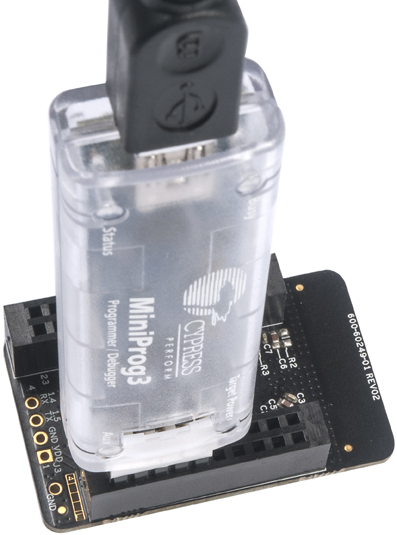
\includegraphics[width=0.25\linewidth]{figures/dongle_miniprog.jpg}
	\caption{Connecting BLE dongle to MiniProg3}
	\label{fig:dongle_prog}
\end{figure}

Steps:
\begin{enumerate}
	\item Build the project (right click on project name > Build \texttt{BLE\_DONGLE}).
	\item Set \texttt{BLE\_DONGLE} project to active (right click on project name > Set As Active Project).
	\item Connect MiniProg to dongle and the PC (see Figure \ref{fig:dongle_prog}).
	\item Program the dongle (\textit{program} button in PSoC creator or Ctrl+F5).
	\item If prompted, select a device to program.
\end{enumerate}

\section{Programming BLE board}

BLE module can be programmed using MiniProg. The code is provided in \texttt{BLE\_UART\_BRIDGE} project of PSoC creator \texttt{MU31S-000} workspace.

\begin{figure}[htb]
    \centering
	  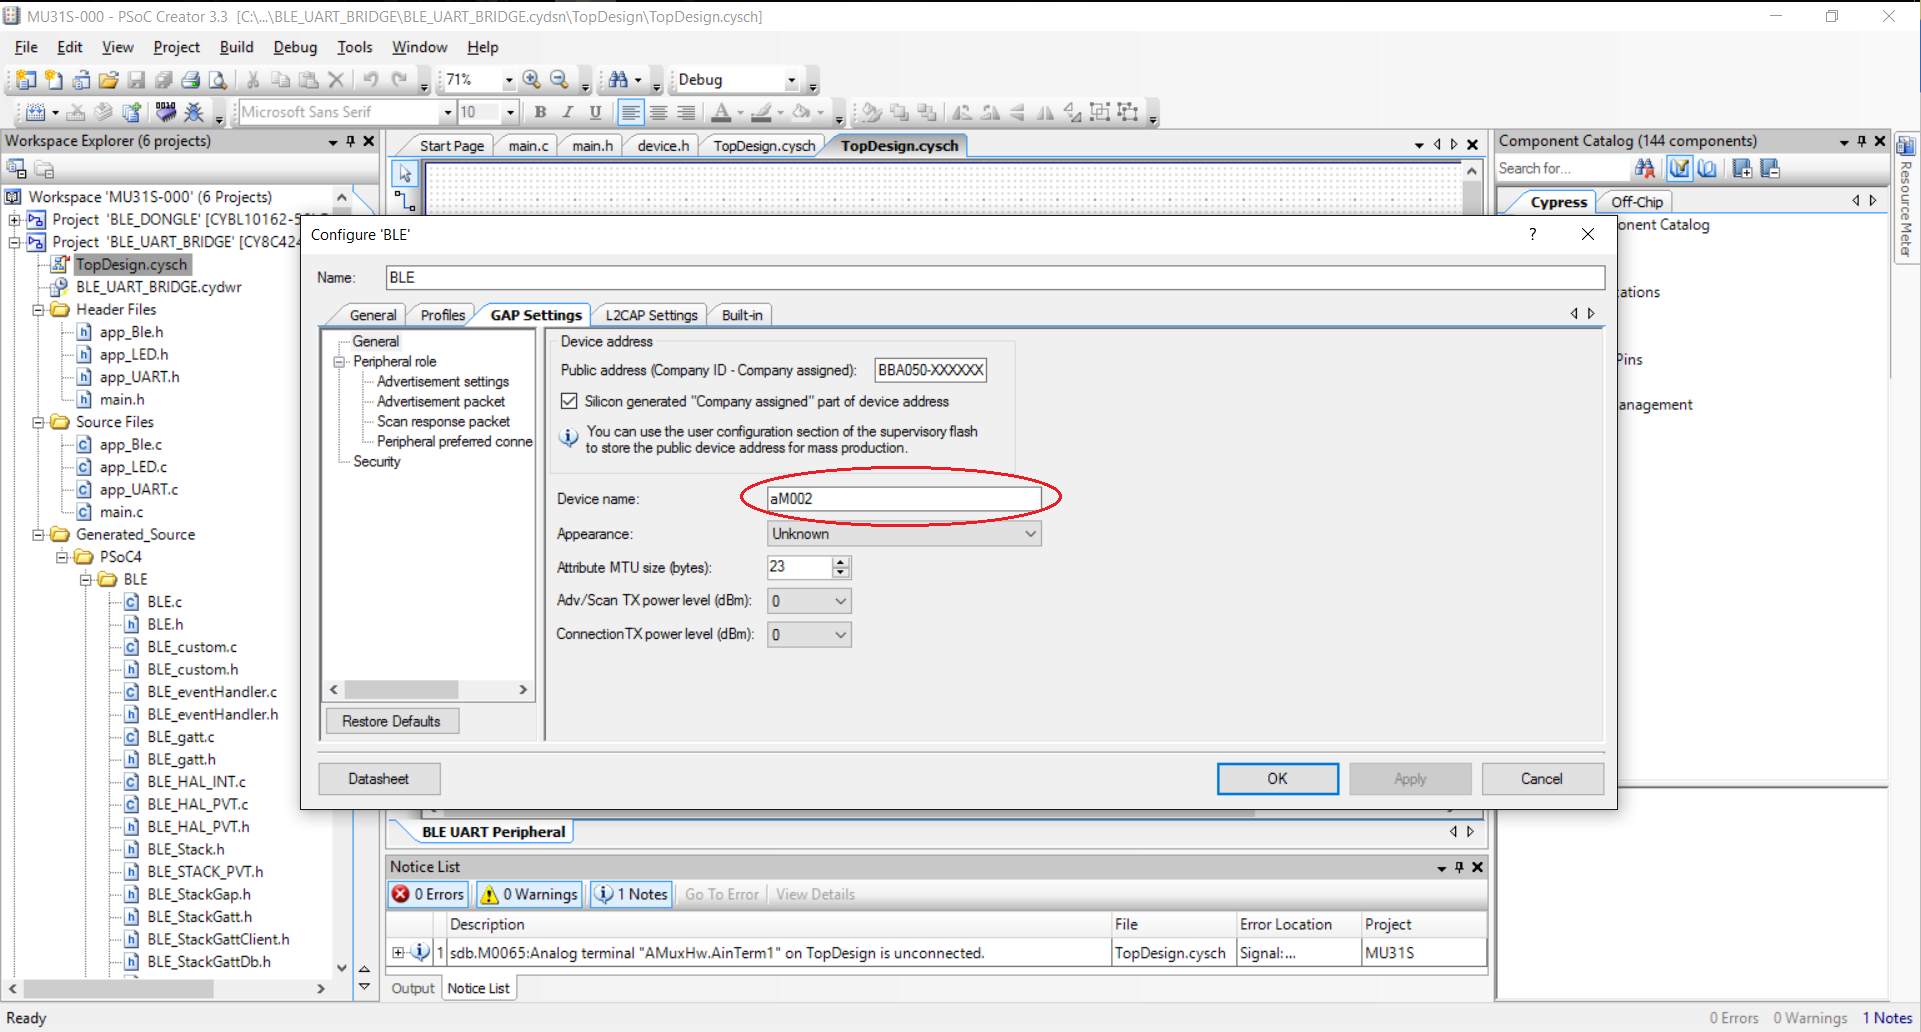
\includegraphics[width=\linewidth]{figures/BLE_device_name.PNG}
	\caption{Setting the BLE device name}
	\label{fig:ble_device_name}
\end{figure}

Steps:
\begin{enumerate}
	\item Modify the project to define aMussel ID. To do so, open TopDesign.cysch and double click on BLE module. Go to GAP Settings > General and enter aMussel ID in Device Name field (see Figure \ref{fig:ble_device_name}). Naming convention is as follows: \texttt{'aMXXX'}, where \texttt{'XXX'} represents aMussel ID in range $[000-999]$, e.g. \texttt{'aM001', 'aM023'} \ldots
	\item Build the project (right click on project name > Build \texttt{BLE\_UART\_BRIDGE}).
	\item Set \texttt{BLE\_UART\_BRIDGE} project to active (right click on project name > Set As Active Project).
	\item Connect MiniProg to BLE board and the PC.
	\item Program the device (\textit{program} button in PSoC creator or Ctrl+F5).
	\item If prompted, select a device to program.
\end{enumerate}

\section{Communicating with MU using BLE}

\begin{figure}[htb]
    \centering
	  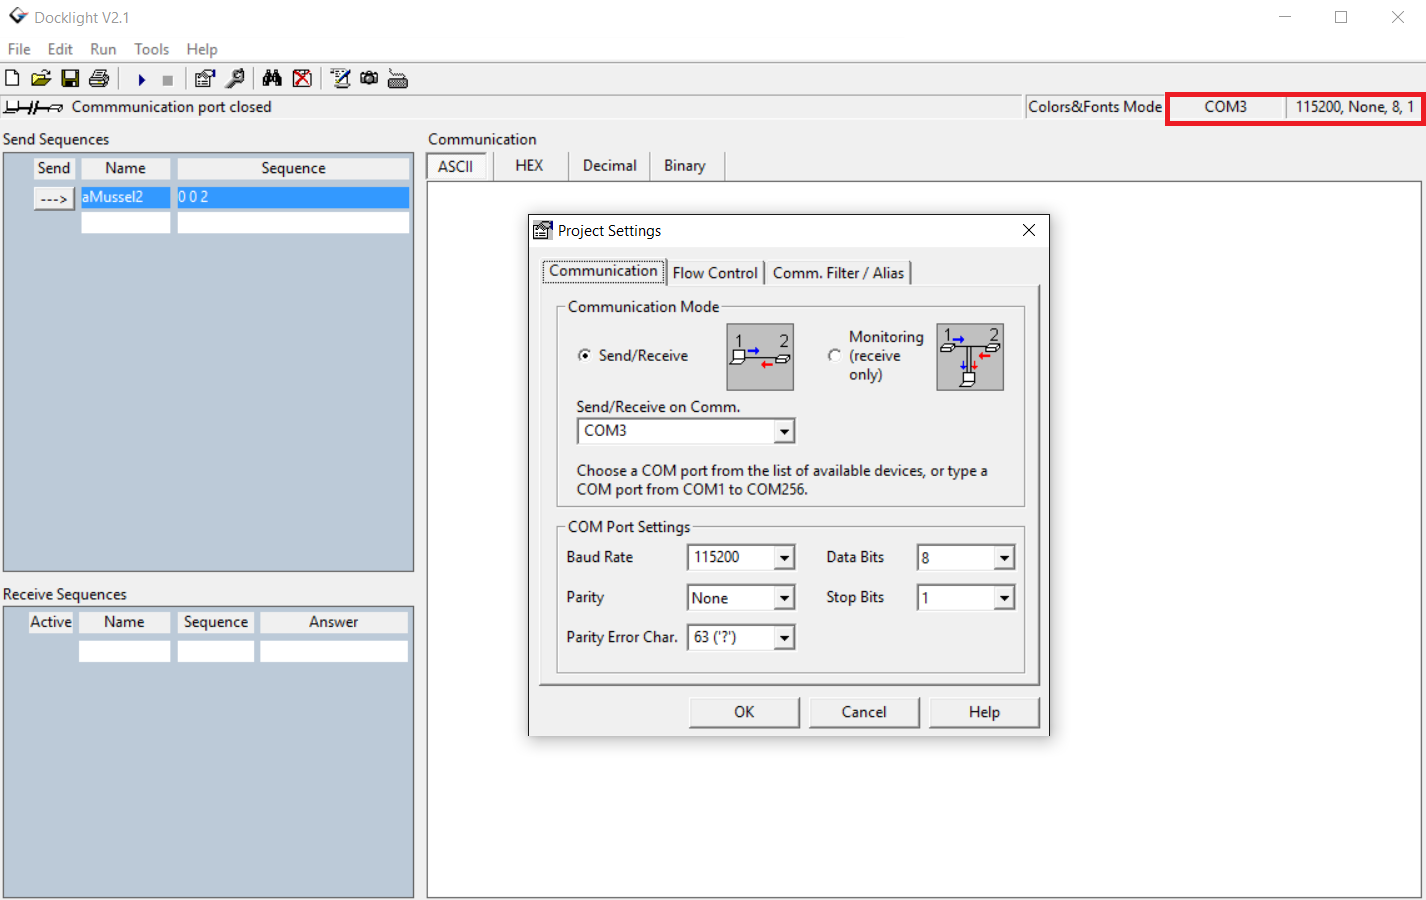
\includegraphics[width=\linewidth]{figures/Docklight_COM.PNG}
	\caption{Selecting the COM port}
	\label{fig:docklight_com}
\end{figure}

\begin{figure}[htb]
    \centering
	  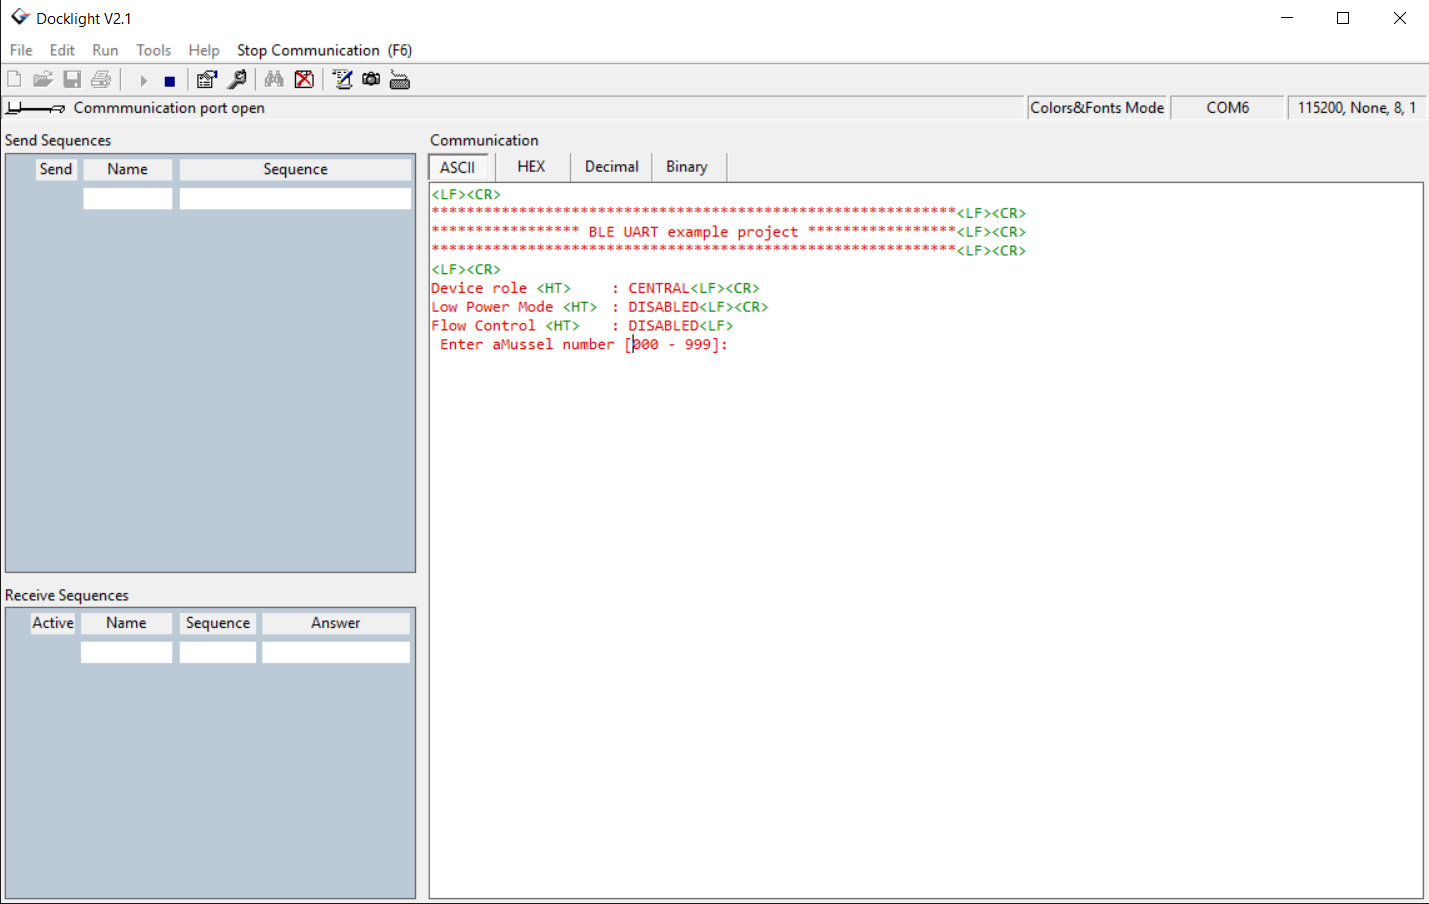
\includegraphics[width=\linewidth]{figures/Docklight_BLE_dongle.PNG}
	\caption{BLE bridge status}
	\label{fig:docklight_ble_bridge_status}
\end{figure}

\begin{figure}[htb]
    \centering
	  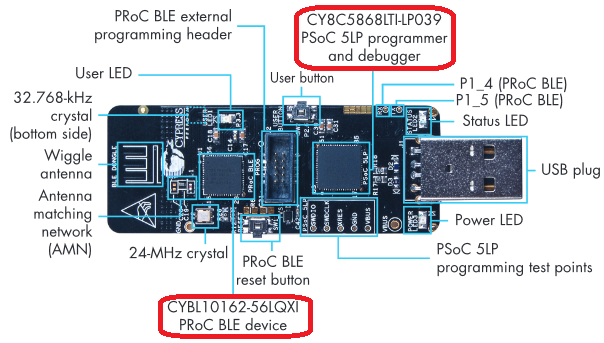
\includegraphics[width=0.6\linewidth]{figures/USB_dongle_parts.png}
	\caption{CY5670 USB Dongle}
	\label{fig:usb_dongle_parts}
\end{figure}

\begin{figure}[htb]
    \centering
	  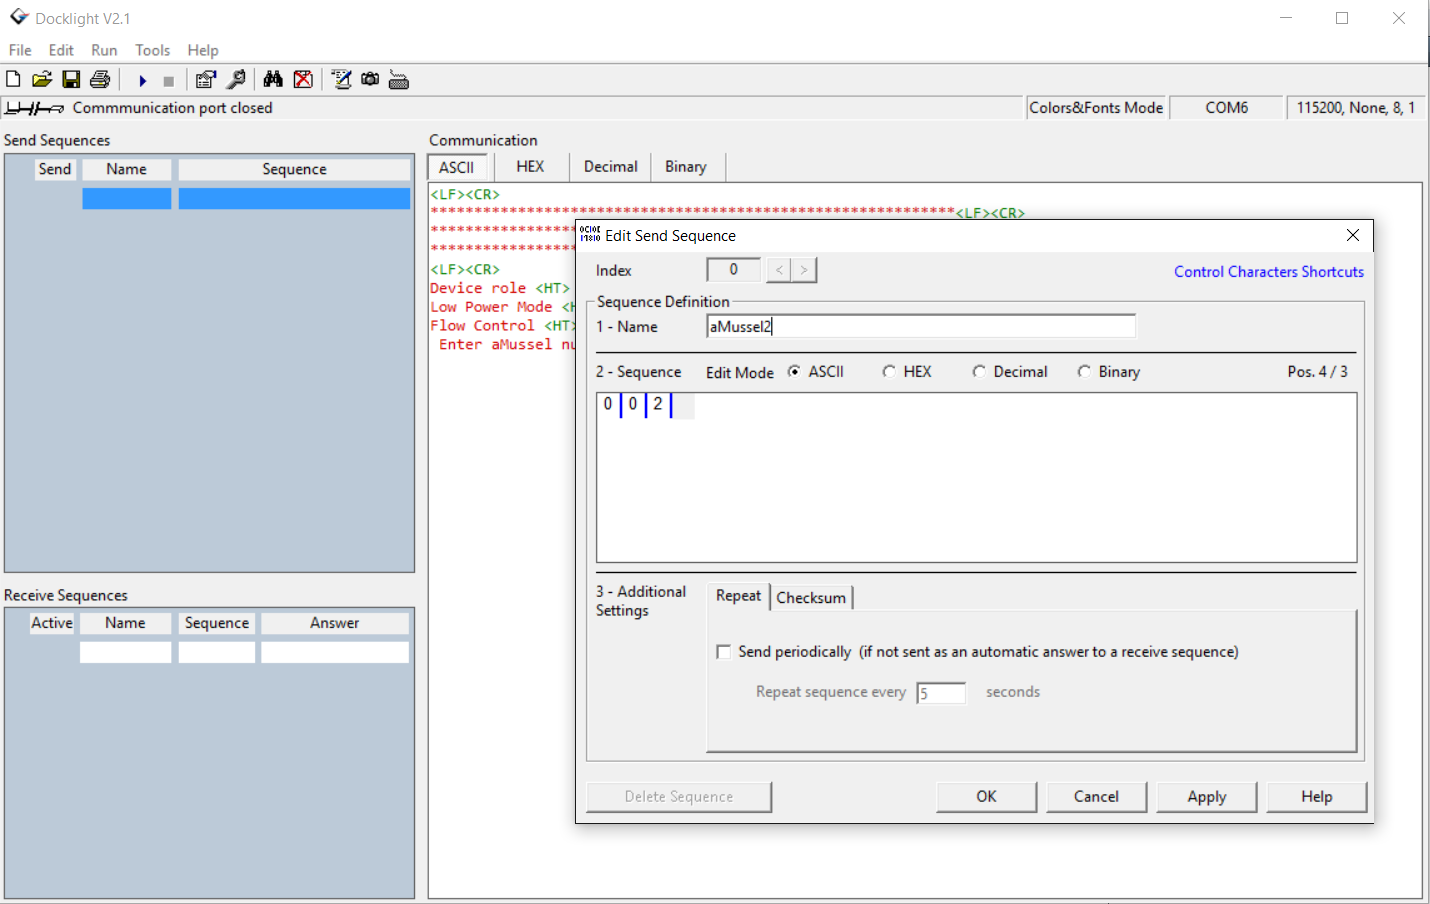
\includegraphics[width=\linewidth]{figures/Docklight_aMussel_selection.PNG}
	\caption{Selecting a device to connect to}
	\label{fig:docklight_aMussel_selection}
\end{figure}

To successfully send and receive data from BLE module on MU, we recommend the following setup:
\begin{enumerate}
	\item Connect programmed BLE dongle to your PC.
	\item Open Docklight \footnote{\url{docklight.de/}} (or any other tool for serial communication).
	\item Connect to the correct COM port. Port can be selected by double clicking on top right sections of status bar (indicated with red rectangle in Figure \ref{fig:docklight_com}). After selecting the port, make sure the settings are matching the ones in the figure. Now you can simply press the play button to establish connection.
	\item When connected to BLE dongle, you should see the output in your serial communication program as presented in Figure \ref{fig:docklight_ble_bridge_status}. If the output is not there or the program is stuck for any reason, you can always reset it by pressing the user button on dongle (see Figure \ref{fig:usb_dongle_parts}).
	\item The next step is to select device ID you wish to connect to. You do so by sending a sequence representing device's unique identifier. For example, if BLE board on aMussel is programmed to have ID \texttt{001}, the sequence needs to match it. For reference, look at Figure \ref{fig:docklight_aMussel_selection}.
	\item Upon connection establishment the program prints out: \\
	\hspace{10pt}\parbox[t]{\linewidth}{\texttt{Server with matching custom service discovered... \\
		Connection established \\
		Notifications enabled \\
		Start entering data:
	}}
	\item Now the connection is established and you can start sending and receiving data.
\end{enumerate}
